% !TEX root = _individual/flatland.tex

%%%%%%%%%%%%%%%%%%%%%%%%%%%%%%%%%%%%%%%%%%%%%%%%%%%%%%%%%%%%%%%%%%%%%%%%%%%%%%%%
\chapter{Flatland Geometry}

Flatland geometry is a fictional two-dimensional space where particles are
constrained to the page \cite{Abb1884,Asa2008}. This differs from standard 2-D
geometry, which represents a 3-D problem that is invariant in the $z$ axis,
where particles can travel at different polar angles out of the page. The
constraint of living in the page reduces the phase space of the transport
equation, as the flatland solution is only a function of the azimuthal angle
$\theta$
rather than both azimuthal and polar angles $\mu,\theta$. This reduction in
phase space makes 
flatland geometry a computationally less burdensome testing ground for new
methods.

Despite being easier computationally to solve, flatland has a few subtle quirks
that need to be understood before a flatland-geometry solver is implemented.
Previous work in flatland \cite{Asa2008,Lar2009c} has shown that the
diffusion coefficient for flatland geometry $\frac{1}{2\sigma}$ is different from
the physical diffusion coefficients $\frac{1}{3\sigma}$, but the correct
formulation for flatland diffusion boundary
conditions have remained an unanswered and indeed unasked question. This
chapter answers that question in addition to providing other insights into this
strange geometry.

%%%%%%%%%%%%%%%%%%%%%%%%%%%%%%%%%%%%%%%%%%%%%%%%%%%%%%%%%%%%%%%%%%%%%%%%%%%%%%%%
\section{Transport in flatland}
To aid in understanding the effect of the geometric constraints on the
diffusion approximation, we write the steady-state transport equation with
isotropic scattering as
\begin{subequations} \label{eqs:ssTransport}
\begin{equation}\label{eq:ssTransportVol}
  \vec{\Omega}\vd \grad I(\vec{x}, \vec{\Omega})
  + \sigma(\vec{x}) I(\vec{x}, \vec{\Omega})
  = \frac{1}{\omega_0} \phi(\vec{x}) \,,
  \quad \vec{x} \in V \,,\ \vec{\Omega} \in \Omega\,.
\end{equation}
Here, we use
\begin{align*}
  I(\vec{x},\vec{\Omega}) &= \text{the steady-state angular intensity,} \\
  \vec{\Omega} &= \text{the angular variable,} \\
  \Omega &= \text{the domain of the angular variable,} \\
  \omega_n &= \text{the $n$th moment of the angular variable, and} \\
  \phi(\vec{x}) &= \text{the scalar intensity, the first angular moment of $I$.}
\end{align*}
The angular domains and definitions are defined in
Table~\ref{tab:angularDomain}, and the moments $\omega_0$ are evaluated in
Table~\ref{tab:angularMoments}. We consider a specified incident
boundary condition:
\begin{equation} \label{eq:ssBndy}
  I(\vec{x}, \vec{\Omega}) = I^b(\vec{x}, \vec{\Omega})
  \quad \vec{x} \in \partial V \,,\ \vec{\Omega} \vd \vec{n} < 0\,.
\end{equation}
\end{subequations}


\begin{table}[htb]
  \centering
  \begin{tabular}{rccc}
\toprule
   Geometry & $\vec{\Omega}$ & Domain $\Omega$ & $\ud\Omega$
\\ \midrule
   1D & $\mu$ & $-1 \le \mu \le 1$ & $\ud\mu$
   \\
   2D & $\sqrt{1-\mu^2} \cos \theta \vec{i}
   + \sqrt{1-\mu^2} \sin \theta \vec{j}$
   & $-1 \le \mu \le 1$, $0 \le \theta < 2\pi$ & $\ud\mu \ud \theta$
   \\
   Flatland & $\cos \theta \vec{i} + \sin \theta \vec{j}$
   & $0 \le \theta < 2\pi$ & $\ud \theta$
   \\
   3D & $\mu \vec{i}
   + \sqrt{1-\mu^2} \cos \theta \vec{j}
   + \sqrt{1-\mu^2} \sin \theta \vec{k}$
   & $-1 \le \mu \le 1$, $0 \le \theta < 2\pi$ & $\ud\mu \ud \theta$
\\ \bottomrule
  \end{tabular}
  \caption{Angular domains of the various geometries.}
  \label{tab:angularDomain}
\end{table}

\begin{table}[htb]
  \centering
  \begin{tabular}{rccc}
\toprule
   Geometry
   & $\omega_0 \equiv \int_\Omega \ud\Omega$
   & $\omega_1 \equiv \int_\Omega \abs{\vec{\Omega}\vd\vec{i}} \ud\Omega$
   & $\omega_2 \equiv \int_\Omega (\vec{\Omega}\vd\vec{i})^2 \ud\Omega$
\\ \midrule
   1D & 2 & 1 & $\frac{2}{3}$
   \\
   2D & $4\pi$ & $2\pi$ & $\frac{4\pi}{3}$
   \\
   Flatland & $2\pi$ & $4$ & $\pi$
   \\
   3D & $4\pi$ & $2\pi$ & $\frac{4\pi}{3}$
\\ \bottomrule
  \end{tabular}
  \caption{Angular moments in each geometry.}
  \label{tab:angularMoments}
\end{table}

%%%%%%%%%%%%%%%%%%%%%%%%%%%%%%%%%%%%%%%%
\subsection{An insightful comparison problem}
To help understand the differences between flatland geometry and real life, we
consider a simple purely absorbing transport problem that describes particles
being emitted from one surface toward another.
This is not a novel problem, so we will not labor over the derivation or
results.

On paper, the problem looks like Fig.~\ref{fig:chordFlatland}. In 2D, the two
gray surfaces and the gap extend infinitely into and out of the page.
In the figure, $\theta$ is the azimuthal angle in both flatland and 2-D
geometry. In flatland, the line of length $s$ is constrained to the plane,
whereas in 2D, $s$ extends out of the plane (see Fig.~\ref{fig:chordXy}).

For the purposes of comparison, we also view Fig.~\ref{fig:chordFlatland} as a
sagittal section of an infinite cylinder; Fig.~\ref{fig:chordRz} shows a
cross-sectional view.

\begin{figure}[htb]
  \centering
  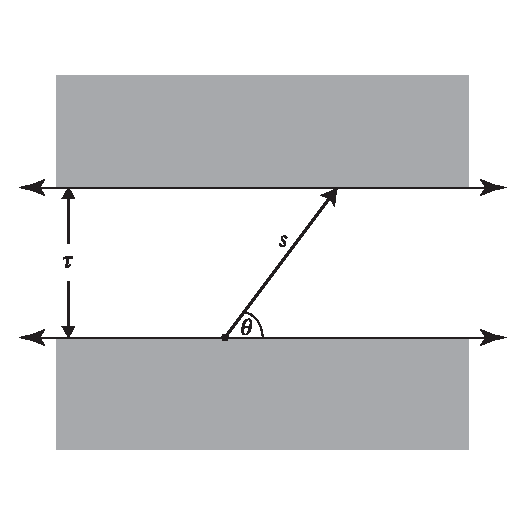
\includegraphics{chord-flatland}
  \caption[The chord length problem as represented on paper.]%
  {The chord length problem as represented on paper. The gap is
  $\tau$ mean free paths apart, $\theta$ is the azimuthal angle, and $s$ is the
  distance across the gap.}
  \label{fig:chordFlatland}
\end{figure}

\begin{figure}[htb]
  \centering
  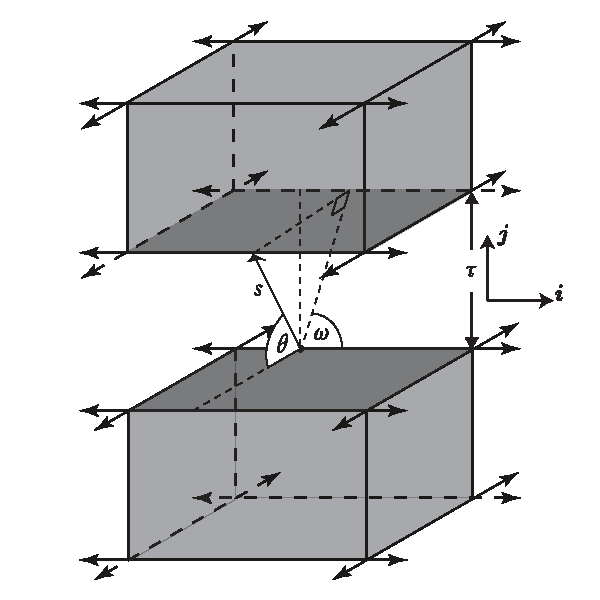
\includegraphics{chord-xyz}
  \caption[A more full view of the chord length problem in 2-D geometry.]%
  {A more full view of the chord length problem in 2-D geometry.
  The polar angle cosine is $\mu= \cos \varphi$, and the azimuthal angle is
  $\theta$.}
  \label{fig:chordXy}
\end{figure}

\begin{figure}[htb]
  \centering
  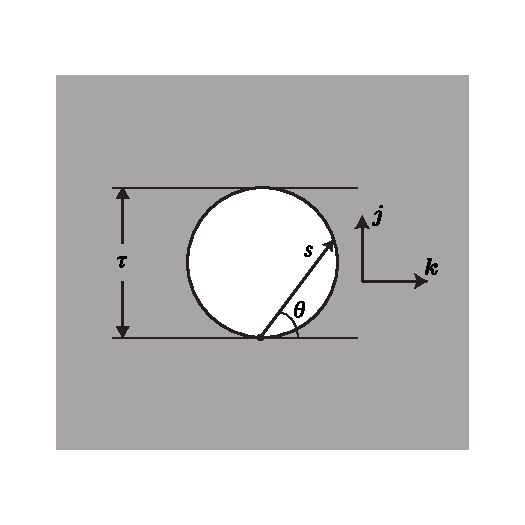
\includegraphics{chord-rz}
  \caption[A cross-section of the chord length problem in cylindrical
  geometry.]%
  {A cross-section of the chord length problem in cylindrical
  geometry. The orthogonal view looks like Fig.~\ref{fig:chordFlatland}.}
  \label{fig:chordRz}
\end{figure}

\subsubsection{Derivation}

The average probability of being emitted isotropically from the surface and
reaching the other side, $\tau$ mean free paths away, without collision is
\begin{align*}
  p(\tau) = \int_{\vec{\Omega}\vd\vec{n}>0} \eexp^{-\tau s(\vec{\Omega}) }
  f(\vec{\Omega}) \ud\Omega\,.
\end{align*}
Here, $f(\vec{\Omega})\ud\Omega$ is the probability of being emitted
isotropically from a surface into $\ud\Omega$ about $\vec{\Omega}$, and $s$ is
the distance to the other side along $\vec{\Omega}$ in units of $\tau$. The
derivation of $f$ will be discussed in \S\ref{sec:isoSurface}.

In flatland, simple geometry relates $s = 1/\sin\theta$, giving
\begin{equation*}
  p(\tau) = \int_{0}^{\pi} \eexp^{-\tau / \sin \theta} \frac{\sin \theta}{2}
  \ud\theta\,.
\end{equation*}

In 2D, the polar direction modifies the length of $s$ by $\sqrt{1-\mu^2}$, and
a coordinate transform from $\vec{j}$ to $\vec{k}$ allows us to re-express the
integral as a simpler function of just $\mu$:
\begin{equation*}
  p(\tau) = \int_{0}^{\pi} \int_{-1}^{1} \eexp^{-\tau / \left(
  \sqrt{1-\mu^2} \sin\theta \right)}
  \frac{\sqrt{1-\mu^2} \sin\theta}{\pi} \ud\mu \ud \theta
  = 2 \int_{0}^{1} \eexp^{-\tau / \mu} \mu \ud\mu\,.
\end{equation*}

For cylindrical geometry, we consider $\theta$ in the cross-sectional plane
(Fig.~\ref{fig:chordRz}) to give the equivalent problem of a circle in 2-D
geometry.
\begin{equation*}
  p(\tau) = \int_{0}^{\pi} \int_{-1}^{1} \eexp^{-\tau \sin \theta / 
  \sqrt{1-\mu^2}}
  \sqrt{1-\mu^2} \frac{\sin\theta}{\pi} \ud\mu \ud \theta\,.
\end{equation*}

\clearpage
\subsubsection{Results}
Evaluating those three probabilities for different values of $\tau$ gives
Table~\ref{tab:collision}. The effect of ``living on the page'' is to have, on
average, a shorter distance across a material, leading to a larger survival
probability.

\begin{table}[htb]
  \centering
  \begin{tabular}{clll}
\toprule
\phantom{10}$\tau$ & \rz & Flatland & \xy
\\ \midrule
          \phantom{0}0.01 & 0.990 & 0.985 & 0.981 \\
\phantom{0}0.1\phantom{0} & 0.906 & 0.863 & 0.833 \\
\phantom{0}1.\phantom{00} & 0.404 & 0.274 & 0.219 \\
10.\phantom{00} & 0.00772 & 1.63\EE{-5} & 7.10\EE{-6}
 \\
\bottomrule
  \end{tabular}
  \caption{Comparison of the probability of crossing a channel $\tau$ mfp thick
  without colliding.}
  \label{tab:collision}
\end{table}

Not sure if this problem was too helpful. Maybe I should just keep the figures
differentiating flatland from 2D and leave out the problem, probabilities, and
results.

%%%%%%%%%%%%%%%%%%%%%%%%%%%%%%%%%%%%%%%%
\subsection{Monte Carlo sampling}
The Monte Carlo method approximates the transport equation by tracking the
random lives of statistically large numbers of particles as they traverse a
problem. The behavior during their lifetime depends on probability distribution
functions (PDFs) that describe how they are born, how far they travel without a
collision, how they behave when they collide, and so on. 

The general Monte Carlo process has been covered extensively elsewhere
\cite{Lew1984,Bro2004a}; our focus in this section is to expound upon the
distributions particular to flatland geometry. We briefly derive those PDFs,
integrate them to get cumulative distribution functions
(CDFs), and use the direct inversion method to show how a pseudo-random number
generator (PRNG) may be used to determine particle behavior in flatland.

\subsubsection{Isotropic volume source}
A particle emitted from an isotropic internal source, whether an extraneous
radiation source or an indirect isotropic scattering event, has an equal
probability of entering any angle. In any geometry, the normalized PDF that
represents this process is
\begin{equation}\label{eq:volumeSource1}
  f(\vec{\Omega}) \ud \Omega = c \ud \Omega \,,
  \quad \vec{\Omega} \in \Omega \,,
\end{equation}
where (see Table~\ref{tab:angularDomain}) $\Omega$ is the angular domain of the
geometry.
Requiring the PDF to integrate to unity over its domain gives the
geometry-independent normalization constant $c$:
\begin{align*}
  1 = \int_{\Omega} f(\vec{\Omega}) \ud\Omega
  = c \int_{\Omega} \ud\Omega
  \lra
  c = \frac{1}{\omega_0}\,.
\end{align*}
Thus the angular distribution of an isotropic volume source is
\begin{equation}\label{eq:volumeSource2}
  f(\vec{\Omega}) \ud \Omega = \frac{\ud\Omega}{\omega_0} \,,
  \quad \vec{\Omega} \in \Omega\,.
\end{equation}

In 2D, using the identities from Tables~\ref{tab:angularDomain}
and~\ref{tab:angularMoments}, Eq.~\eqref{eq:volumeSource2} evaluates to the
familiar
\begin{equation*}
  f(\mu,\theta) \ud\mu\ud\theta = \frac{\ud\mu\ud\theta}{4\pi} 
  = \frac{\ud\mu}{2}\frac{\ud\theta}{2\pi}
  \,,
  \quad -1\le \mu \le 1,\ 0 \le \theta < 2\pi\,,
\end{equation*}
which gives the separable CDF
\begin{equation*}
  F(\mu,\theta) = F_1(\mu) F_2(\theta)
  = \frac{1 + \mu}{2}\frac{\theta}{2\pi}\,,
  \quad -1\le \mu \le 1,\ 0 \le \theta < 2\pi\,.
\end{equation*}
Setting $\xi_1 = F(\mu)$, $\xi_2 = F(\theta)$, solving for $\mu,\theta$, and
introducing them back into the 2-D representation of $\vec{\Omega}$, we get the
well-known result
\begin{equation*}
  \vec{\Omega} = \sqrt{1-\mu^2} \cos \theta \vec{i}
   + \sqrt{1-\mu^2} \sin \theta \vec{j}
  = \sqrt{1-(2\xi_1-1)^2} \cos(2\pi\xi_2) \vec{i}
   + \sqrt{1-(2\xi_1-1)^2} \sin(2\pi\xi_2) \vec{j}\,.
\end{equation*}

In flatland, Eq.~\eqref{eq:volumeSource2} becomes the simpler
\begin{equation*}
  f(\theta) \ud\theta = \frac{\ud\theta}{2\pi} \,,
  \quad 0 \le \theta < 2\pi\,,
\end{equation*}
yielding the CDF
\begin{equation}\label{eq:volumeSourceFlatland}
  F(\theta) = \frac{\theta}{2\pi}\,,
  \quad 0 \le \theta < 2\pi\,,
\end{equation}
Setting $\xi_1 = F(\theta)$ and solving for $\theta = F\inv(\xi_1)$ gives the
simple result that
\begin{equation*}
  \theta = 2\pi \xi_1\,.
\end{equation*}
The flatland particle's new angle is therefore
\begin{equation*}
  \vec{\Omega} = \cos \theta \vec{i} + \sin \theta \vec{j}
  = \cos(2\pi\xi_1) \vec{i} + \sin(2\pi\xi_1) \vec{j}\,.
\end{equation*}

With only one independent variable that needs sampling, and the omission of
the transcendental operation $\sqrt{1-\mu^2}$, the computational cost of a
scattering event is significantly less in flatland than in 2D, leading to
faster simulation times.

\subsubsection{Isotropic surface source}\label{sec:isoSurface}
Particles emitted from an isotropic surface source have a cosine distribution
\cite{Gre2002}, which makes constant the radiation flux in each differential
angle:
\begin{equation}\label{eq:surfaceSource1}
  f(\vec{\Omega}) \ud \Omega = c \abs{\vec{\Omega}\vd \vec{n}} \ud \Omega \,,
\quad \vec{\Omega}\vd \vec{n} < 0 \,,
\end{equation}
where $c$ is a normalization constant.

Requiring the PDF to integrate to unity over its domain gives the
normalization constant independent of geometry:
\begin{align*}
  1 &= \int_{\vec{\Omega}\vd \vec{n} < 0} f(\vec{\Omega}) \ud\Omega
  \\
  1 &= c \int_{\vec{\Omega}\vd \vec{n} < 0} \abs{\vec{\Omega}\vd \vec{n}}
    \ud\Omega
  \\
  1 &=\frac{c}{2} \int_{\Omega} \abs{\vec{\Omega}\vd \vec{n}} \ud\Omega
  \\
  c &= \frac{2}{\omega_1}\,.
\end{align*}
With this, the PDF for an isotropic surface source,
Eq.~\eqref{eq:surfaceSource1}, becomes
\begin{equation}\label{eq:surfaceSource2}
  f(\vec{\Omega}) \ud \Omega = \frac{2}{\omega_1} \abs{\vec{\Omega}\vd \vec{n}} \ud \Omega \,,
\quad \vec{\Omega}\vd \vec{n} < 0 \,.
\end{equation}
In 3D, choosing $\vec{n}=\vec{i}$, this PDF is
\begin{equation*}
  f(\mu,\theta) \ud\mu \ud\theta
  = \frac{1}{\pi} \mu \ud\mu \ud\theta
  = (2 \mu \ud\mu) \frac{\ud\theta}{2\pi}\,,
\end{equation*}
which gives the separable CDF
\begin{equation*}
  F(\mu,\theta) = (\mu^2) \frac{\theta}{2\pi}\,,
\end{equation*}
from which we can sample $\mu=\sqrt{\xi_1}$ and $\theta=2\pi \xi_2$.

In flatland, the surface source distribution is different. Let us choose
$\vec{n} = -\vec{j}$ so that incident directions are inside
$\theta \in [0, \pi)$.
Applying the flatland identities in Tables~\ref{tab:angularDomain}
and~\ref{tab:angularMoments} to Eq.~\eqref{eq:surfaceSource1} gives the surface
source PDF of
\begin{equation*}
  f(\theta) \ud\theta = \frac{2}{4} \, \abs{ -\sin \theta}\ud\theta
  = \frac{1}{2} \sin \theta\ud\theta \,,\quad 0 \le \theta < \pi\,.
\end{equation*}
Integrating, we find the CDF for particle emission from
a surface source in flatland geometry to be
\begin{equation}\label{eq:surfaceSourceFlatland}
  F(\theta) = \frac{1}{2} \left( 1-\cos\theta \right)
  \,,\quad 0 \le \theta < \pi\,,
\end{equation}
Solving for $\theta = F\inv(\xi_1)$ gives a sampled angle for a surface source
in flatland:
\begin{equation*}
  \theta = \cos\inv(1 - 2\xi_1)\,.
\end{equation*}
Finally, we insert this into the flatland $\vec{\Omega}$ and use the identity
$\cos^2 \theta + \sin^2 \theta = 1$ to reduce the number of transcendental
functions. The direction of a particle from an isotropic surface source is
\begin{align*}
  \vec{\Omega} &= \cos \theta \vec{i} + \sin \theta \vec{j} \\
  &=  \cos[ \cos\inv(1 - 2\xi_1) ] \vec{i} + \sin[ \cos\inv(1 - 2\xi_1) ] \vec{j} \\
  &= (1 - 2\xi_1) \vec{i} + \sqrt{1 - (1 - 2\xi_1)^2} \vec{j}\,.
\end{align*}

%%%%%%%%%%%%%%%%%%%%%%%%%%%%%%%%%%%%%%%%
\subsection{Discrete ordinates quadrature}

A standard practice in two-dimensional discrete ordinates (\SN)
solvers is to create a quadrature set that only creates polar
angles for the top half of a unit sphere, $\mu>0$, and to modify
the ordinate weights to sum to $4\pi$ \cite{Zik1997}.

%%%%%%%%%%%%%%%%%%%%%%%%%%%%%%%%%%%%%%%%%%%%%%%%%%%%%%%%%%%%%%%%%%%%%%%%%%%%%%%%
\section{Diffusion in flatland}

In 2-D geometry, particles diffuse in three dimensions, although their density
is projected onto the 2-D plane. In contrast, flatland particles have one fewer
dimension into which to leak: as we will see, the result is a larger diffusion
coefficient.

The differences in the identities shown in Table~\ref{tab:angularMoments}
result not
only in a different diffusion coefficient but also different boundary
conditions. In this section, we derive boundary conditions from a steady-state
transport equation with isotropic scattering. There is no loss of generality in
ignoring the time dependence because of the quasi-static approximation made in
the derivation of the diffusion coefficient (see \S\ref{sec:diffusion}).

To aid the reader in understanding whence the different coefficients in the
diffusion equation arise, we use the geometric constants given in
Table~\ref{tab:angularMoments},
\begin{equation*}
  \omega_n \equiv \int_\Omega \abs{\vec{\Omega} \vd \vec{i}}^n \ud \Omega\,,
\end{equation*}
where $\Omega$ is the domain of the angular variable $\vec{\Omega}$. In 2-D,
$\vec{\Omega}$ sweeps the $4\pi$ unit sphere and is projected to the plane, but
in flatland, $\vec{\Omega}$ lives on a $2\pi$ unit circle.

%%%%%%%%%%%%%%%%%%%%%%%%%%%%%%%%%%%%%%%%
\subsection{Interior diffusion approximation}

The diffusion approximation begins by assuming that $I$ is linear in angle:
\begin{equation*}
  I(\vec{x}, \vec{\Omega}) \approx f(\vec{x}) + \vec{\Omega} \vd
  \vec{g}(\vec{x})\,.
\end{equation*}
The zeroth angular moment of $I$ determines $f$:
\begin{equation*}
  \phi = \int_\Omega I \ud \Omega
= \int_\Omega \left( f + \vec{\Omega}\vd \vec{g} \right) \ud\Omega
= \int_\Omega\ud\Omega f + 0
= \omega_0 f \,,
\end{equation*}
so $f = \phi/\omega_0$. Similarly, the first moment of $I$ gives $g$:
\begin{equation*}
  \vec{F} = \int_\Omega \vec{\Omega} I \ud \Omega
= f \int_\Omega \vec{\Omega} \ud\Omega
  + \vec{g} \vd \int_\Omega \vec{\Omega}\vec{\Omega} \ud\Omega
= \omega_2 \vec{g} \,,
\end{equation*}
so $\vec{g} = \vec{F}/\omega_2$. This is the \Pone\ approximation for $I$ in the different geometries:
\begin{equation}\label{eq:ssPone}
  I(\vec{x}, \vec{\Omega})
  \approx \frac{1}{\omega_0} \phi(\vec{x})
  + \frac{1}{\omega_2} \vec{\Omega} \vd \vec{F}(\vec{x})\,.
\end{equation}

The diffusion approximation is a closure for the first angular moment of
the transport equation, so we now operate on Eq.~\eqref{eq:ssTransportVol} with
$\int_\Omega \vec{\Omega} (\cdot) \ud \Omega$ and substitute
Eq.~\eqref{eq:ssPone}:
\begin{align*}
  \grad \vd \int_\Omega \vec{\Omega} \vec{\Omega} I
  \ud\Omega
  + \sigma \int_\Omega \vec{\Omega} I \ud\Omega
  &= \frac{1}{\omega_0} \phi(\vec{x}) \int_\Omega \vec{\Omega} \ud\Omega
  \\
  \grad \vd \int_\Omega \vec{\Omega} \vec{\Omega} I(\vec{x}, \vec{\Omega})
  \ud\Omega
  + \sigma \vec{F}
  &= 0
  \\
  \grad \vd \int_\Omega \vec{\Omega} \vec{\Omega} \left(
  \frac{1}{\omega_0}\phi + \frac{1}{\omega_2} \vec{\Omega} \vd \vec{F}
  \right) \ud\Omega
  + \sigma \vec{F}
  &= 0
  \\
  \frac{1}{\omega_0} \grad \vd \int_\Omega \vec{\Omega} \vec{\Omega}
  \ud\Omega \phi 
  + \sigma \vec{F} &= 0
  \\
  \frac{\omega_2}{\omega_0} \grad \phi + \sigma \vec{F} &= 0 \,.
\end{align*}
Solving for $\vec{F}$ gives Fick's law, expressed in the general-geometry form:
\begin{equation} \label{eq:fickGeneral}
  \vec{F}(\vec{x})
  = - \frac{\omega_2}{\omega_0} \frac{1}{\sigma(\vec{x})} \grad \phi(\vec{x})
  \equiv -D(\vec{x}) \grad \phi(\vec{x})\,.
\end{equation}
In 2-D and 3-D, $\omega_2/\omega_0 = (4\pi / 3) / (4\pi) = 1/3$; however, in
flatland, $\omega_2/\omega_0 = \pi / (2\pi) = 1/2$. Thus, $D=(3\sigma)\inv$ in
2-D but $D=(2\sigma)\inv$ in flatland.

Substituting Fick's law back into the linear-in-angle approximation,
Eq.~\eqref{eq:ssPone}, we get the diffusion approximation to the angular
intensity:
\begin{align} \nonumber
  I(\vec{x}, \vec{\Omega})
  &\approx \frac{1}{\omega_0} \phi(\vec{x})
  + \frac{1}{\omega_2} \vec{\Omega} \vd \left[ - \frac{\omega_2}{\omega_0}
  \frac{1}{\sigma(\vec{x})} \grad \phi(\vec{x}) \right]\,.
  \\ \label{eq:diffusionIntensity}
  I(\vec{x}, \vec{\Omega})
  &= \frac{1}{\omega_0} \left[ \phi(\vec{x})
  - \frac{1}{\sigma(\vec{x})}
  \vec{\Omega} \vd \grad \phi(\vec{x}) \right] \,.
\end{align}
In 2-D, Eq.~\eqref{eq:diffusionIntensity} evaluates to the standard result
\begin{equation*}
 I(\vec{x}, \vec{\Omega})
= \frac{1}{4\pi} \left[ \phi(\vec{x}) - \frac{1}{\sigma(\vec{x})} \vec{\Omega}
\vd \grad \phi(\vec{x}) \right] \,,
\end{equation*}
and in flatland, it is
\begin{equation}\label{eq:flatlandDiffusion}
 I(\vec{x}, \vec{\Omega})
= \frac{1}{2\pi} \left[ \phi(\vec{x}) - \frac{1}{\sigma(\vec{x})} \vec{\Omega}
\vd \grad \phi(\vec{x}) \right]\,.
\end{equation}

%%%%%%%%%%%%%%%%%%%%%%%%%%%%%%%%%%%%%%%%
\subsection{Marshak boundary condition}
The Marshak boundary condition \cite{Mar1947} preserves the incident radiation
flux on the boundary. It is derived by substituting the approximate diffusion
intensity from Eq.~\eqref{eq:diffusionIntensity} into the boundary condition,
Eq.~\eqref{eq:ssBndy}, multiplying by $\abs{\vec{\Omega}\vd \vec{n}}$, and integrating over
incident directions.
\begin{align*}
\int_{\vec{\Omega}\vd \vec{n} < 0 } \abs{\vec{\Omega}\vd \vec{n}}
I^b \ud\Omega
 &= 
\int_{\vec{\Omega}\vd \vec{n} < 0 } \abs{\vec{\Omega}\vd \vec{n}} 
 \frac{1}{\omega_0} \left[ \phi - \frac{1}{\sigma}
  \vec{\Omega} \vd \grad \phi \right]
  \ud\Omega
\\
F^{-}
&= 
\frac{1}{\omega_0} \phi \left( \int_{\vec{\Omega}\vd \vec{n} < 0 }
\abs{\vec{\Omega}\vd \vec{n}} \ud\Omega \right) 
  - \frac{1}{\omega_0}\frac{1}{\sigma}
  \int_{\vec{\Omega}\vd \vec{n} < 0 } (-\vec{\Omega}\vd \vec{n})
  \vec{\Omega} \ud\Omega  \vd \grad \phi
\\
F^{-}
&=
\frac{1}{\omega_0} \phi \left( \frac{\omega_1}{2} \right) 
  + \frac{1}{\omega_0}\frac{1}{\sigma} \vec{n} \vd
  \int_{\vec{\Omega}\vd \vec{n} < 0 } \vec{\Omega} \vec{\Omega} \ud\Omega
  \vd \grad \phi
\\
F^{-}
&=
\frac{\omega_1}{2\omega_0} \phi 
  + \frac{1}{\omega_0}\frac{1}{\sigma} \vec{n} \vd
  \left( \int_{\vec{\Omega}\vd \vec{n} < 0 } \vec{\Omega} \vec{\Omega} \ud\Omega \right)
  \vd \grad \phi
\\
F^{-}
&=
\frac{\omega_1}{2\omega_0} \phi
+ \frac{1}{\omega_0}\frac{1}{\sigma} \vec{n} \vd \left( \frac{\omega_2}{2}
\Identitytens \right) \grad \phi
\\
F^{-}
&=
\frac{\omega_1}{2\omega_0} \phi
+ \frac{\omega_2}{2\omega_0}\frac{1}{\sigma} \vec{n} \vd \grad \phi\,.
\end{align*}
Rearranging gives an expression for the Marshak boundary condition for 
\begin{equation} \label{eq:marshak}
\frac{2\omega_0}{\omega_1} F^{-}
=
\phi + \frac{\omega_2}{\omega_1}\frac{1}{\sigma} \vec{n} \vd \grad \phi
\end{equation}

The value
\begin{equation*}
  z_0 \equiv \frac{\omega_2}{\omega_1}
  =
  \begin{cases}
    \frac{2}{3} \approx 0.6667 & \text{1D, 2D, 3D,} \\
    \frac{\pi}{4} \approx 0.7854 & \text{Flatland,}
  \end{cases}
\end{equation*}
is the Marshak extrapolation distance.

Substituting the diffusion coefficient $D$ from Eq.~\eqref{eq:fickGeneral} gives
\begin{equation*}
\frac{2\omega_0}{\omega_1} F^{-}
= \phi + \frac{\omega_0}{\omega_1} D \vec{n} \vd \grad \phi\,.
\end{equation*}
In 1D, 2D, and 3D, this evaluates to
\begin{equation*}
4 F^{-}
= \phi + 2 D \vec{n} \vd \grad \phi\,,
\end{equation*}
but in flatland it is
\begin{equation*}
\pi F^{-}
= \phi + \frac{\pi}{2} D \vec{n} \vd \grad \phi\,.
\end{equation*}

%%%%%%%%%%%%%%%%%%%%%%%%%%%%%%%%%%%%%%%%
\subsection{Variational boundary condition} \label{sec:varBndy}
It is well known that the Marshak boundary condition is not consistent with the
true transport boundary condition. A lengthy asymptotic boundary layer
matching analysis \cite{Hab1975} shows that the correct weighting of the
boundary condition is not $\abs{\vec{\Omega}\vd\vec{n}}$ but rather
$W(\abs{\vec{\Omega}\vd\vec{n}})$, where $W$ is related to Chandrasekhar's
$H$-function \cite{Cha1960}:
\begin{equation} \label{eq:chandraW}
  W(\mu) = \frac{\sqrt{3}}{2} \mu H(\mu) \,.
\end{equation}
In general geometries, this leads to the extrapolation distance of
\begin{align*}
  z_0 = \frac{\int_{0}^{1} \mu W(\mu) \ud \mu}{\int_{0}^{1} W(\mu) \ud
  \mu} \approx 0.7104\,.
\end{align*}

In real-world geometries, a variational analysis \cite{Mal1991} can be used to
derive a very accurate approximation to $W$:
\begin{equation*}
W(\mu) \approx \mu + \tfrac{3}{2} \mu^2 \,,
\end{equation*}
which gives the approximate extrapolation distance of
\begin{equation*}
  z_0 = \frac{\int_{0}^{1} \mu (\mu + \tfrac{3}{2} \mu^2 ) \ud
  \mu}{\int_{0}^{1} (\mu + \tfrac{3}{2} \mu^2 ) \ud \mu} 
  = \frac{17}{24} \approx 0.7083 \,.
\end{equation*}
%This variational analysis can be imitated by taking a semi-infinite,
%source-free, purely scattering transport problem, assuming the exiting $I$ is
%constant in angle, and making a particular demand.

Now we repeat that analysis for flatland rather than real space. The first step
is to consider a homogeneous, purely scattering transport problem in a
semi-infinite plane. The transport equation~\eqref{eq:ssTransportVol} becomes
\begin{subequations} \label{eqs:flatTransport}
\begin{equation}\label{eq:flatTransportVol}
  \cos \theta \pder{I}{x} + \sin \theta \pder{I}{y} + \sigma I
  = \frac{\sigma}{2\pi} \int_{0}^{2\pi} I \ud \theta'\,,\quad
 -\infty < x < \infty,\ 0 \le y < \infty,\ 0 \le \theta < 2\pi\,.
\end{equation}
It has a uniform incident boundary condition,
\begin{equation}\label{eq:flatTransportBndy}
  I(x, 0, \theta) = I^b(\theta) \,,\quad -\infty < x < \infty,\ 
  0 \le \theta < \pi \,.
\end{equation}
\end{subequations}
Also, because there is no variation in the boundary condition or $\sigma$ along
the $x$ axis, $\tpder{I}{x}=0$, and Eq.~\eqref{eq:flatTransportVol} becomes the
one-dimensional transport equation 
\begin{equation*}
  \sin \theta \pder{}{y}I(y,\theta) + \sigma I(y,\theta)
  = \frac{\sigma}{2\pi} \int_{0}^{2\pi} I(y,\theta') \ud \theta'\,.
\end{equation*}
This is \emph{not} the same one-dimensional transport equation as in slab
geometry.

We define the $y$ components of the angular moments of $I$ as
\begin{equation} \label{eq:flatPhi}
  \phi_m(y) = \int_{0}^{2\pi} (\vec{\Omega}\vd\vec{j})^m I(y,\theta) \ud\theta
  = \int_{0}^{2\pi} (\sin\theta)^m I(y,\theta) \ud\theta \,.
\end{equation}

As $y\to\infty$, the intensity $I$ will approach a constant $\varphi/2\pi$,
which gives $\phi_0(\infty)=\varphi$. Concordantly, $\phi_1(\infty)=0$.

Operating on the transport equation with $\int_{0}^{2\pi} (\sin\theta)^m (\cdot)
\ud\theta$ gives the $m$th angular moment in the $y$ direction:
\begin{align} \nonumber
  \pder{}{y} \int_{0}^{2\pi} (\sin\theta)^{m+1} I \ud\theta
  + \sigma \int_{0}^{2\pi} (\sin\theta)^{m} I \ud\theta
  &= \frac{\sigma}{2\pi} \int_{0}^{2\pi} I \ud \theta'
  \int_{0}^{2\pi} (\sin\theta)^{m} \ud\theta
  \\ \label{eq:flatMoments}
  \pder{\phi_{m+1}}{y}
  + \sigma \phi_{m}
  &= \frac{\sigma}{2\pi} \phi_{0}
  \int_{0}^{2\pi} (\sin\theta)^{m} \ud\theta\,.
\end{align}
For $m=0$, the conservation equation, Eq.~\eqref{eq:flatMoments} evaluates to
\begin{equation*}
  \pder{\phi_{1}}{y}
  + \sigma \phi_{0}
  = \frac{\sigma}{2\pi} \phi_{0} (2\pi)
  \lra
  \pder{\phi_{1}}{y} = 0\,.
\end{equation*}
That means the radiation flux is a constant, and because $\phi_1(\infty)=0$,
that constant is zero.

Evaluating Eq.~\eqref{eq:flatMoments} for $m=1$ and using the result that
$\phi_{1}=0$, we find
\begin{equation*}
  \pder{\phi_{2}}{y}
  + \sigma \phi_{1}
  = \frac{\sigma}{2\pi} \phi_{0} (0)
  \lra
  \pder{\phi_{2}}{y} = 0\,.
\end{equation*}
Thus $\phi_{2}$ is also a constant. As $y\to\infty$, $I\to\varphi/2\pi$, so
\begin{equation*}
  \phi_{2} = \int_{0}^{2\pi} (\sin\theta)^2 \frac{\varphi}{2\pi} \ud\theta
  = \frac{1}{2} \varphi\,.
\end{equation*}
% in 1D, this would be $\int_{-1}^{1}\mu^2\frac{\varphi}{2} \ud \mu =
% \frac{1}{3} \varphi$.

Now, since $\phi_1=0$, we can add $\alpha \phi_1$ to this equation for any
$\alpha$:
\begin{align*}
 \alpha\phi_1 + \phi_{2} &= \frac{\varphi}{2} \\
 \int_{0}^{2\pi} (\alpha \sin\theta + \sin^2\theta)
 I(y,\theta) \ud\theta
 &= \frac{\varphi}{2}\,.
\end{align*}
At the boundary $y=0$, $I=I^b$ for incident angles $0 \le \theta < \pi$. The
variational analysis makes the reasonable approximation that, to leading order,
the exiting particles are isotropically distributed, $I(0,\theta)=I^\text{out}$.
\begin{equation*}
 \int_{0}^{\pi} (\alpha \sin\theta + \sin^2\theta)
 I^b(\theta) \ud\theta
 + \int_{\pi}^{2\pi} (\alpha \sin\theta + \sin^2\theta)\ud\theta I^\text{out}
 = \frac{\varphi}{2}\,.
\end{equation*}
The value $\alpha=\pi/4$ eliminates the integral over outgoing directions and
gives a relation between moments of the incident angular intensity and the
magnitude of the intensity as $y\to\infty$:
\begin{equation}\label{eq:varBoundary}
  \int_{0}^{\pi} \left( \frac{\pi}{4} \sin\theta + \sin^2\theta \right)
 I^b(\theta) \ud\theta
 = \frac{\varphi}{2}\,.
\end{equation}

Diffusion in flatland approximates the intensity as 
\begin{equation*}
  I(\vec{x}, \vec{\Omega}) \approx \frac{1}{2\pi} \left[ \phi(\vec{x}) -
  \frac{1}{\sigma(\vec{x})} \vec{\Omega}
\vd \grad \phi(\vec{x}) \right]
\end{equation*}
In our simple transport problem, $\vec{\Omega} \vd \grad \phi=\sin\theta
\pder{\phi_0}{y}$. We wish our boundary condition to preserve the value of
$\varphi$ when the diffusion method is used:
\begin{align*}
 \varphi = 2\int_{0}^{\pi} \left( \frac{\pi}{4} \sin\theta + \sin^2\theta \right)
 I^b(\theta) \ud\theta
 &= 
  2\int_{0}^{\pi} \left( \frac{\pi}{4} \sin\theta + \sin^2\theta \right)
 \left( \frac{1}{2\pi} \phi -
  \frac{1}{\sigma} \sin\theta \pder{\phi_0}{y}\right)\ud\theta
\\
\int_{0}^{\pi} \left( \frac{\pi}{2} \sin\theta + 2 \sin^2\theta \right)
 I^b(\theta) \ud\theta
 &= 
\frac{1}{2\pi} \int_{0}^{\pi} \left( \frac{\pi}{2} \sin\theta + 2 \sin^2\theta
\right)\ud\theta
 \phi -
 \frac{1}{2\pi} \int_{0}^{\pi} \left( \frac{\pi}{2} \sin^2\theta + 2 \sin^3\theta \right)\ud\theta \frac{1}{\sigma} \pder{\phi_0}{y}
  \\
 &= 
 \frac{1}{2\pi} \left( \frac{\pi}{2} [2] + 2 \frac{\pi}{2}
\right) \phi
-
\frac{1}{2\pi} \left( \frac{\pi}{2} \left[ \frac{\pi}{2} \right] + 2 \left[
\frac{4}{3} \right] \right) \frac{1}{\sigma} \pder{\phi_0}{y}
\\
 &= 
  \phi
- \left( \frac{\pi}{8} + \frac{4}{3\pi} \right) \frac{1}{\sigma} \pder{\phi_0}{y}
\,.
\end{align*}
In this problem, we chose a boundary surface normal of $\vec{n}=-\vec{j}$. Now
replacing $\sin \theta$ with $-\vec{\Omega}\vd\vec{n}$, we get the general
boundary condition for flatland diffusion,
\begin{equation} \label{eq:flatlandDiffusionVarBc}
\int_{\vec{\Omega}\vd\vec{n} < 0} \left[ \frac{\pi}{2}
\abs{\vec{\Omega}\vd\vec{n}} + 2 (\vec{\Omega}\vd\vec{n})^2 \right]
I^b(\vec{x}, \vec{\Omega}) \ud\Omega
= 
  \phi(\vec{x})
  - \left( \frac{\pi}{8} + \frac{4}{3\pi} \right) \frac{1}{\sigma}
  \vec{n}\vd\grad \phi(\vec{x})\,.
\end{equation}
Essentially, we have shown that the flatland equivalent of the $W$ function,
which we shall call $V$, can be approximated by
\begin{equation}\label{eq:flatlandVariational}
  V(\theta)
  \approx \frac{1}{4}\sin\theta + \frac{1}{\pi} \sin^2\theta \,,\quad
  0 \le \theta < \pi \,,
\end{equation}
which satisfies
\begin{equation*}
  \int_{0}^{\pi} V(\theta) \ud\theta= 1
\end{equation*}
and gives the extrapolation distance
\begin{equation*}
  z = \frac{\int_{0}^{\pi} \sin \theta V(\theta) \ud\theta}{\int_{0}^{\pi}
  V(\theta) \ud\theta} =  \frac{\pi}{8} + \frac{4}{3\pi} \,.
\end{equation*}
% \left( \frac{3\pi^2 + 32}{24\pi} \right)

%%%%%%%%%%%%%%%%%%%%%%%%%%%%%%%%%%%%%%%%%%%%%%%%%%%%%%%%%%%%%%%%%%%%%%%%%%%%%%%%
\clearpage

``Marshak'' extrapolation distance:
\begin{equation*}
  z = \frac{\pi}{4} \approx 0.78540
\end{equation*}
Variational extrapolation distance:
\begin{equation*}
  z = \frac{\pi}{8} + \frac{4}{3\pi} \approx 0.81711
\end{equation*}

%%%%%%%%%%%%%%%%%%%%%%%%%%%%%%%%%%%%%%%%%%%%%%%%%%%%%%%%%%%%%%%%%%%%%%%%%%%%%%%%
\section{Summary}
The flatland geometry is a fictional geometry that can act as a computationally
cheap test bed for methods development: it retains the spatial complexity of
multi-dimensional problems, yet the angular treatment is easier. In Monte Carlo
implementations, fewer random numbers are sampled per event and fewer expensive
transcendental functions are evaluated. In the discrete ordinates method, only
one azimuthal angle $\mu=0$ needs to be accounted for.

